\documentclass[11pt, a4paper]{article}
\usepackage[utf8]{inputenc}
\usepackage{graphicx}
\usepackage{fancyhdr}
\usepackage{tikz}
\usepackage{float}
\graphicspath{{../}}

\usepackage{gfsartemisia-euler}
\usepackage[T1]{fontenc}

\usepackage{listings}
\usepackage{longtable}

%%%%%%%%%%%%%%%%%%%%%%%%%%%%%%%%%%%%%%%%%%%%%%
%%%%%%%%%%          CONFIG          %%%%%%%%%%
\newcommand{\settingsTitle}{Munin: A Simple Emulator for Execution-Time Memory Complexity Analysis\\\large Fall 2023 CS 335 Final Project}
\newcommand{\settingsFirstName}{Eleftheria}
\newcommand{\settingsLastName}{Beres}
\newcommand{\settingsMonth}{Dec}
\newcommand{\settingsYear}{2023}
\newcommand{\settingsCourseDept}{COMP\_SCI}
\newcommand{\settingsCourseNum}{335} % DON'T FORGET `\_'
\newcommand{\settingsQuarter}{Fall}
%%%%%%%%%%          CONFIG          %%%%%%%%%%
%%%%%%%%%%%%%%%%%%%%%%%%%%%%%%%%%%%%%%%%%%%%%%

% create title
\title{\settingsTitle}
\author{\settingsFirstName\,\settingsLastName}
\date{\settingsMonth\,\settingsYear}

\begin{document}

\twocolumn

% set pagestyle
\pagestyle{fancy}
\setlength{\headheight}{13.59999pt}

% clear header
\fancyhead{}

% set header
\fancyhead[L]{\settingsCourseDept\,\settingsCourseNum\, | \settingsQuarter\,\settingsYear}
\fancyhead[R]{\settingsLastName}

% homework title
\maketitle
% ensure titlepage has same style
\thispagestyle{fancy}

Hello

\begin{figure}[H]
    \centering
    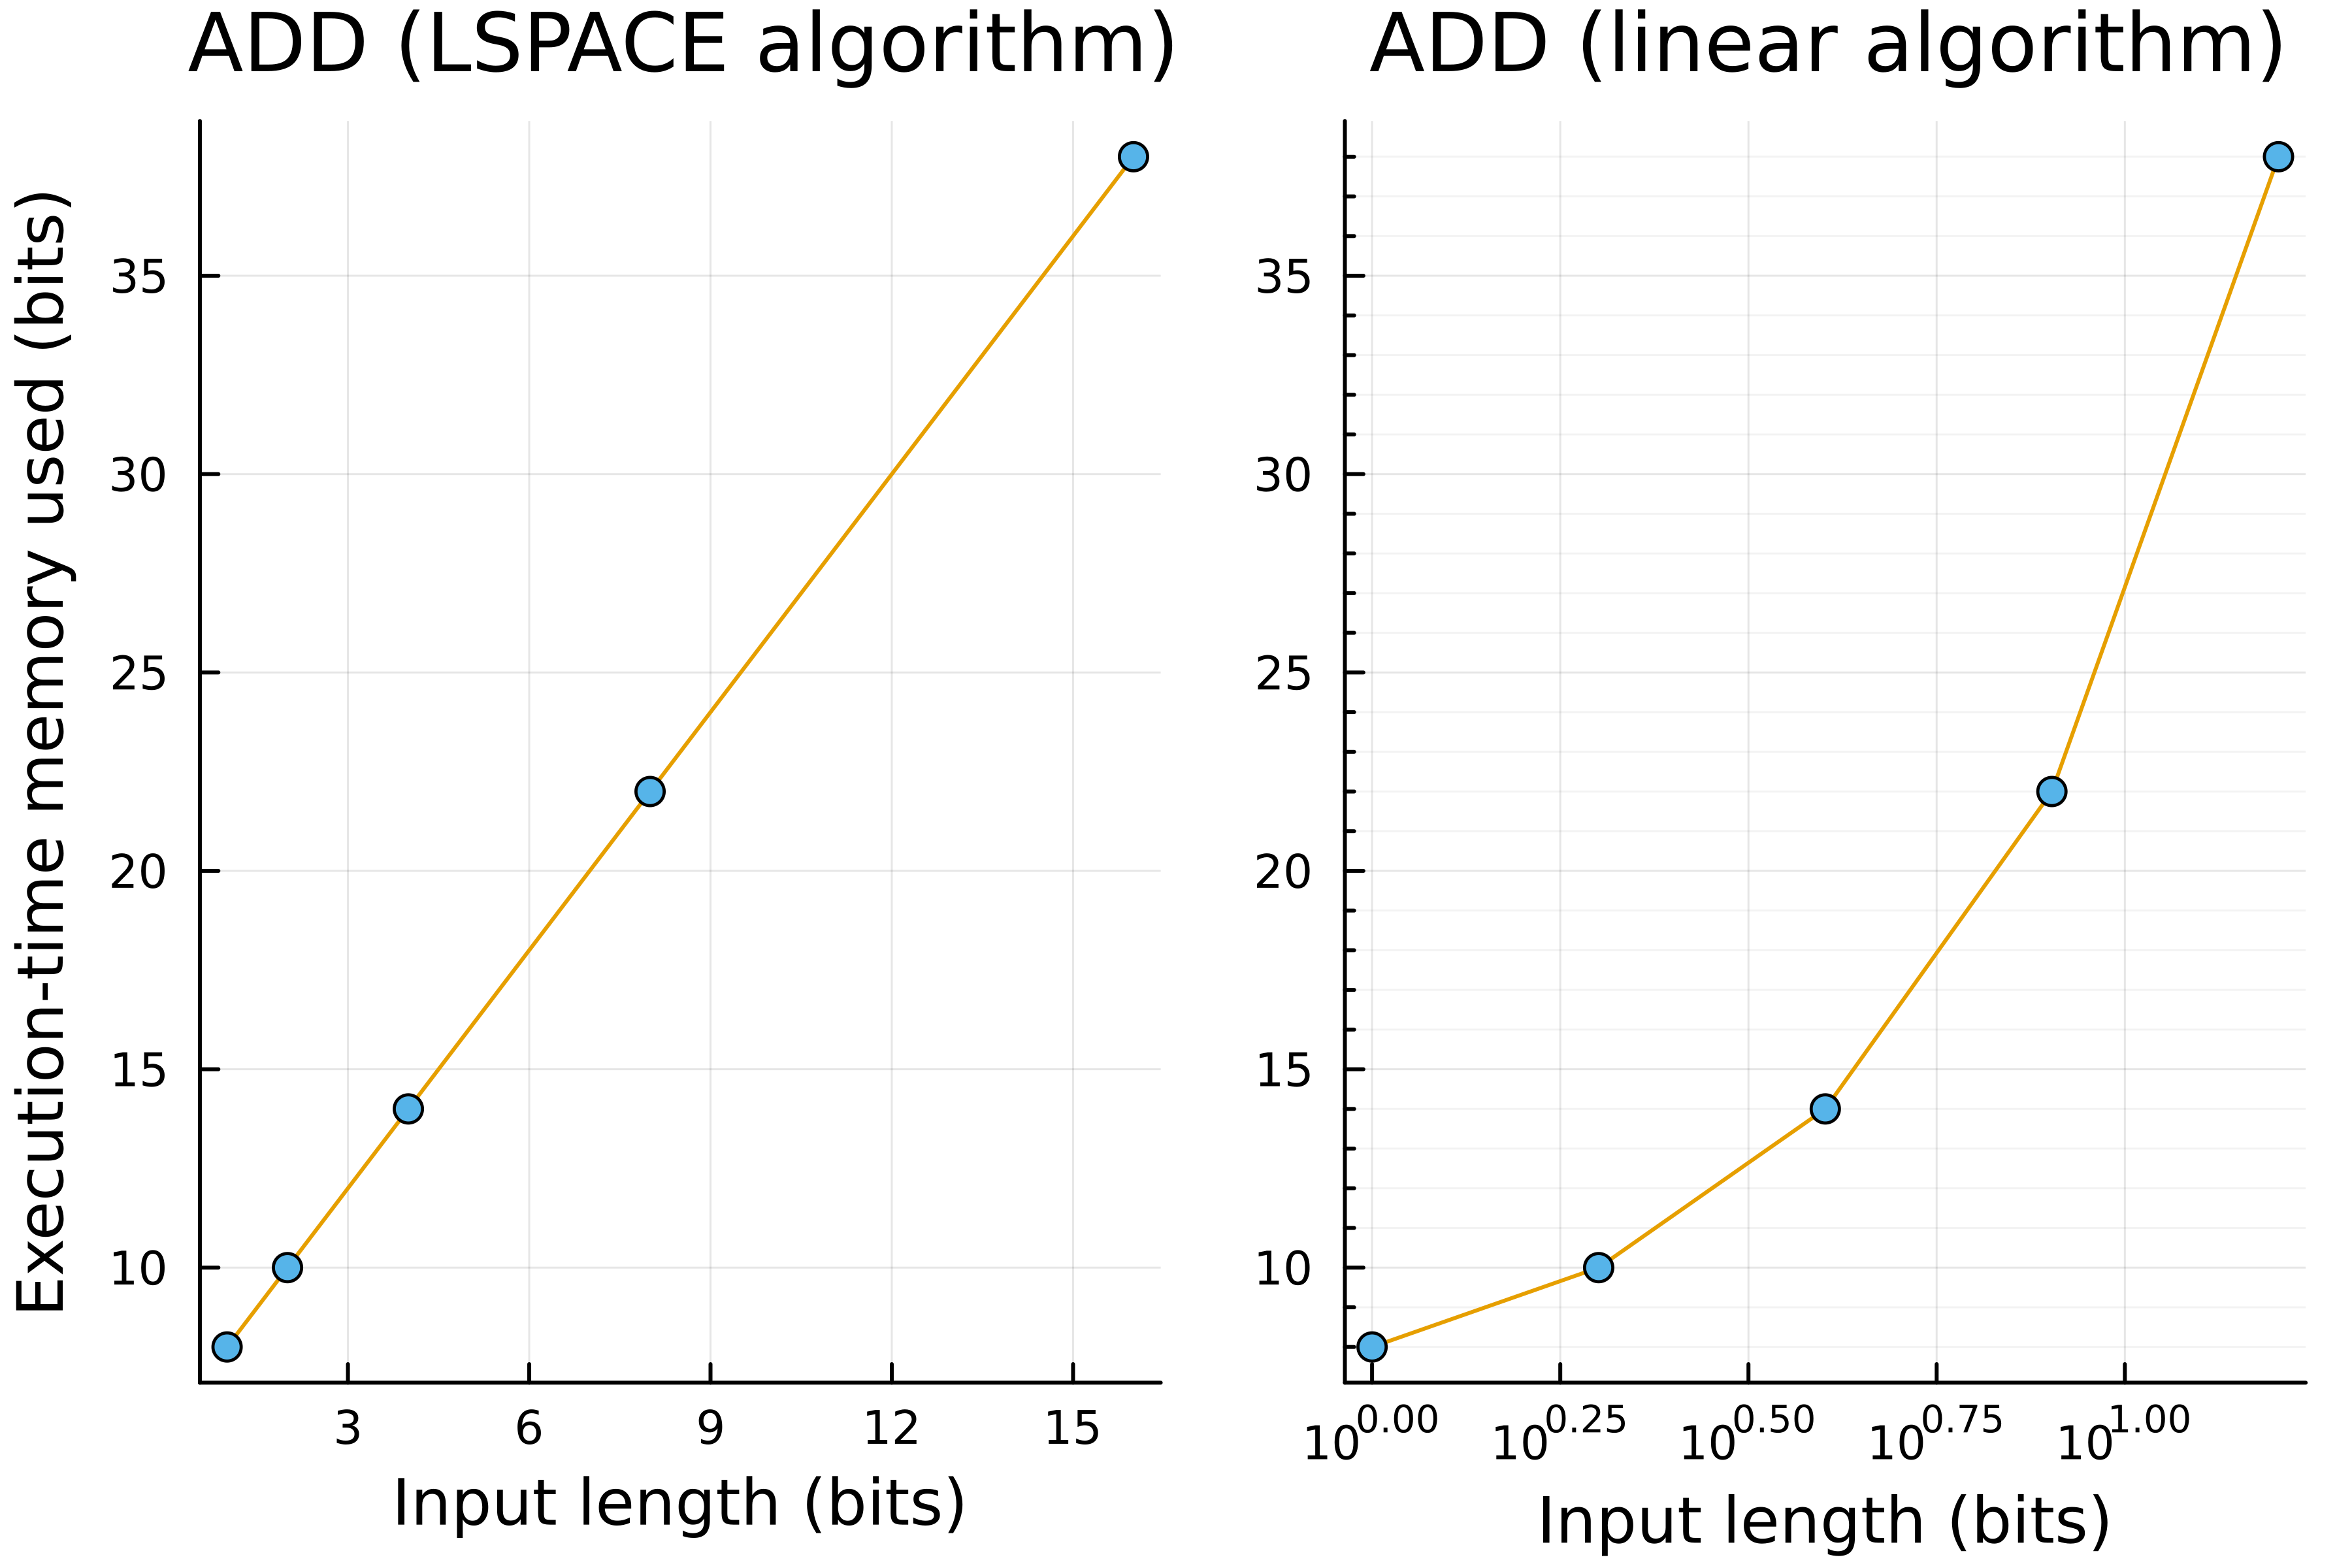
\includegraphics[width=\columnwidth]{ADD-(linear-algorithm).png}
    \caption{Execution-time memory usage (bits) vs. input length (bits) for the linear space ADD algorithm given in Appendix \ref{app:linAdd}}
    \label{fig:linAdd}
\end{figure}

\begin{figure}[H]
    \centering
    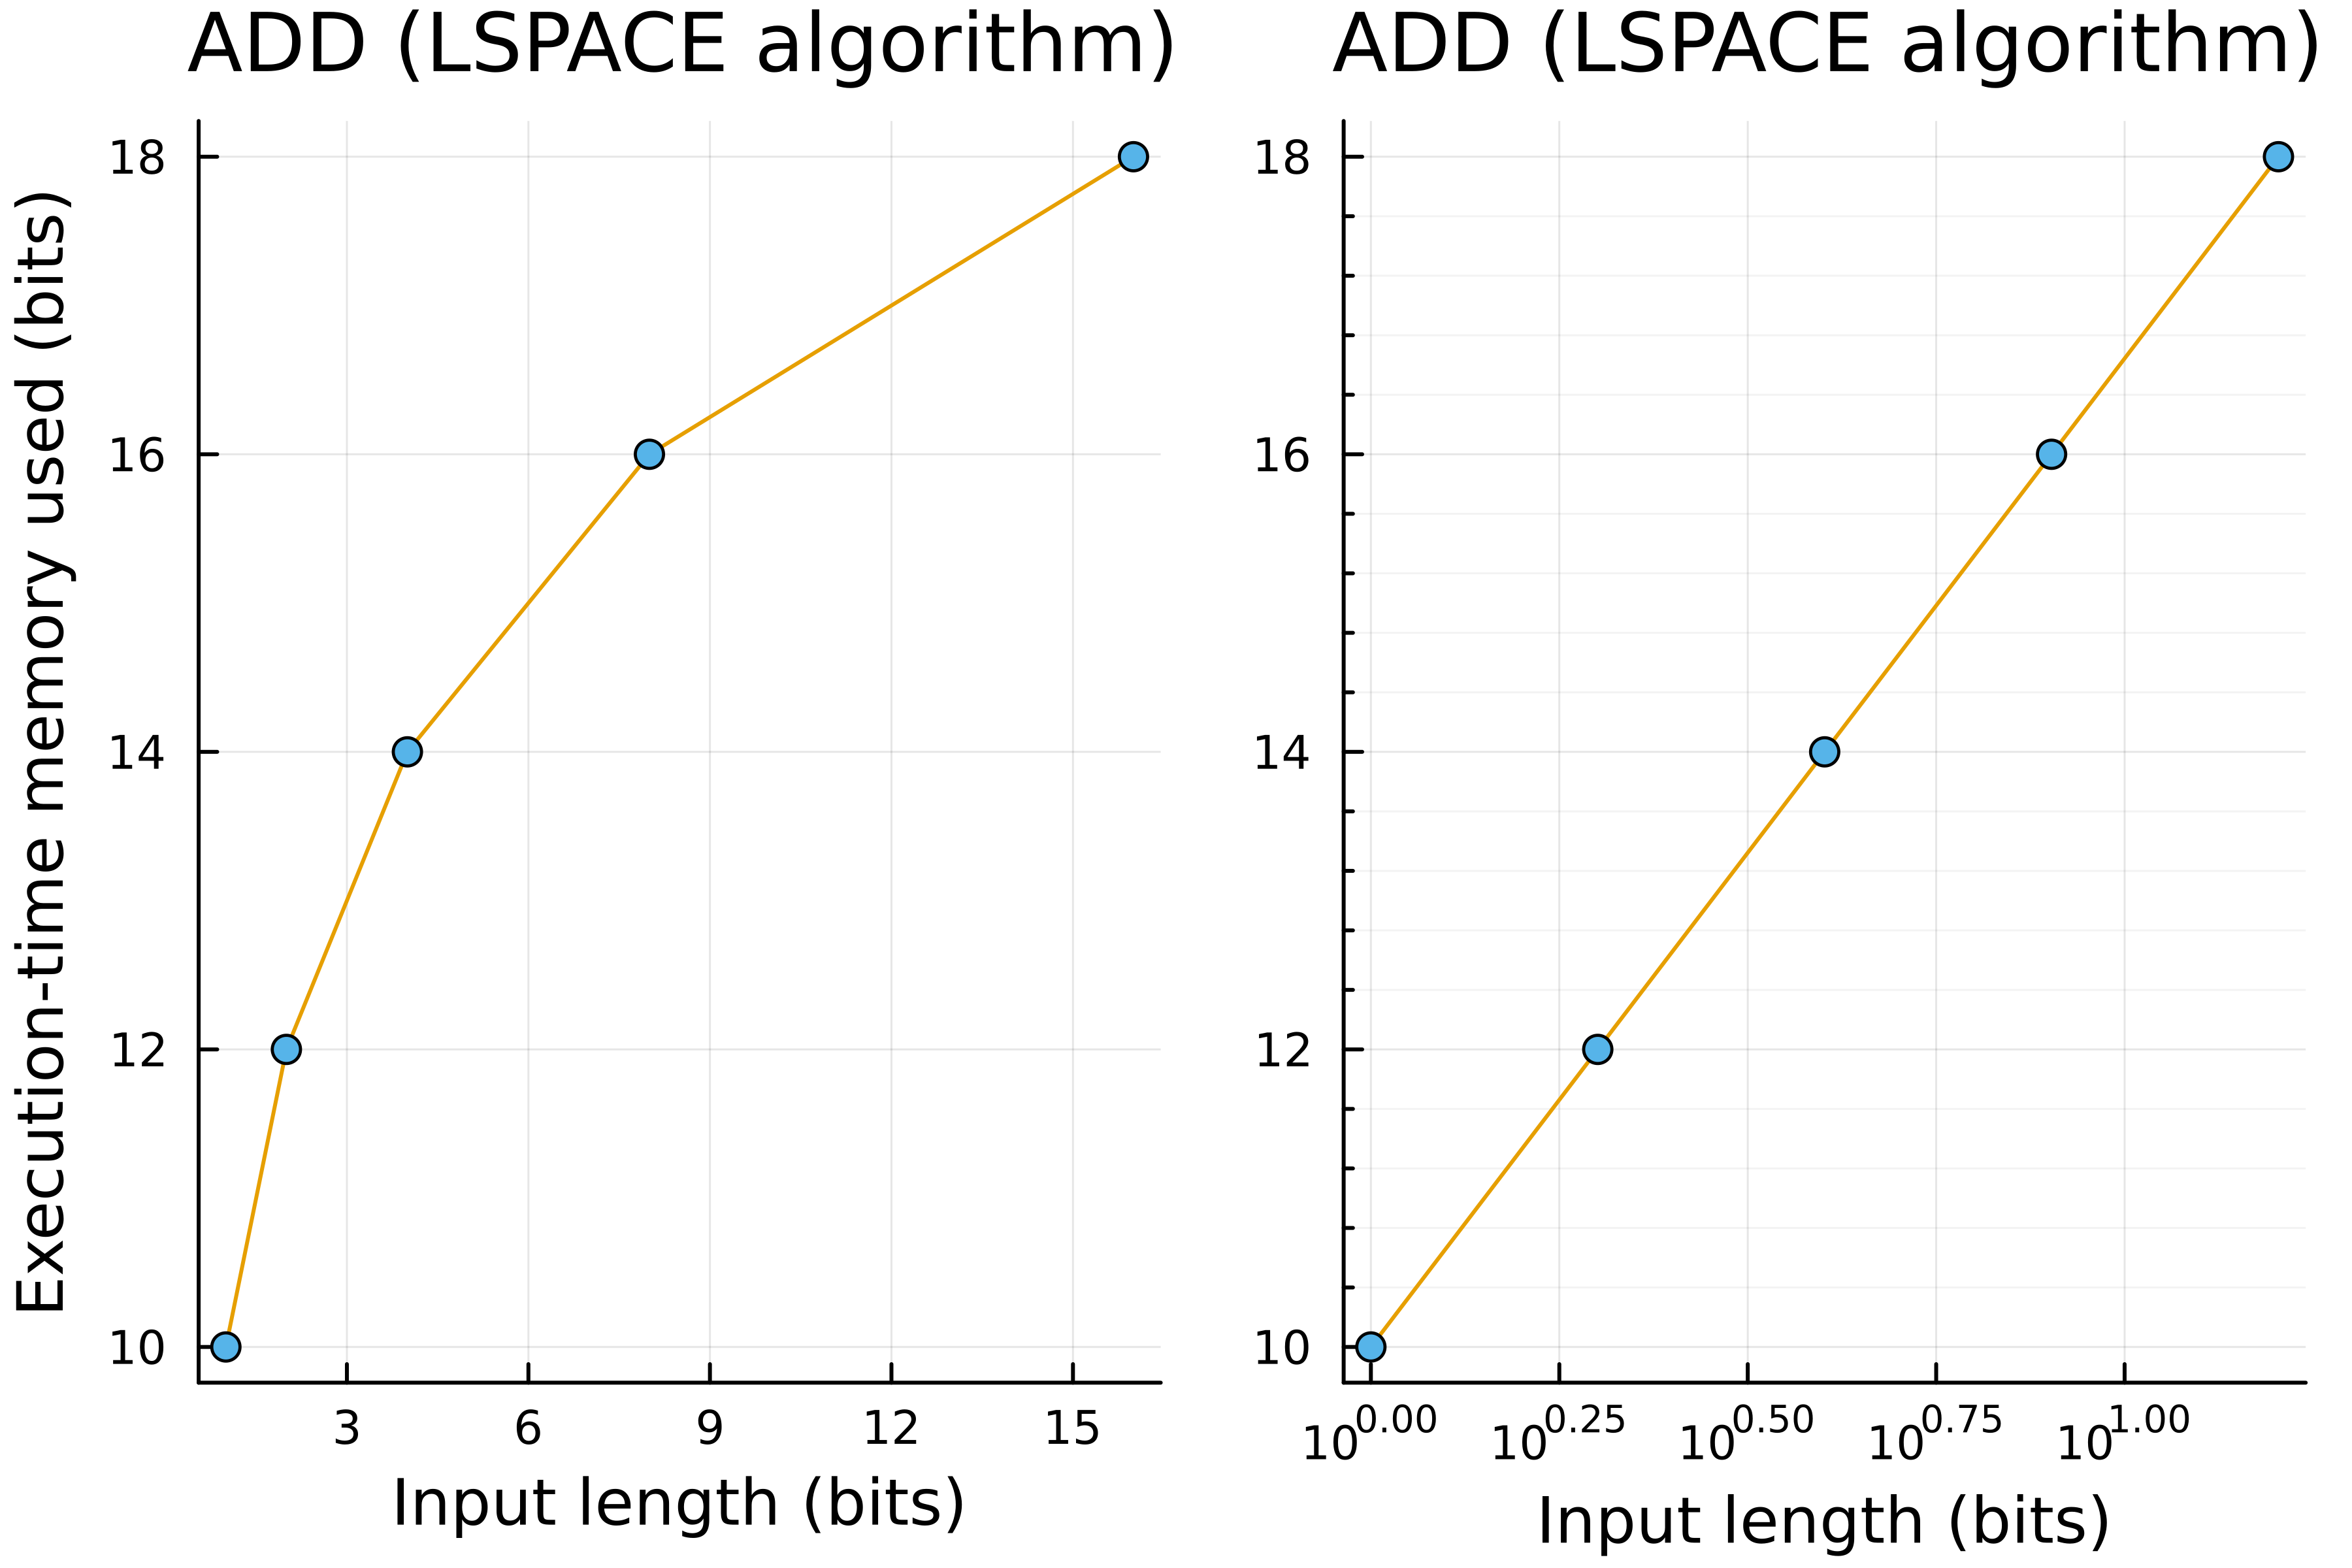
\includegraphics[width=\columnwidth]{ADD-(LSPACE-algorithm).png}
    \caption{Execution-time memory usage (bits) vs. input length (bits) for the LSPACE ADD algorithm given in Appendix \ref{app:lAdd}}
    \label{fig:lAdd}
\end{figure}

\begin{figure}[H]
    \centering
    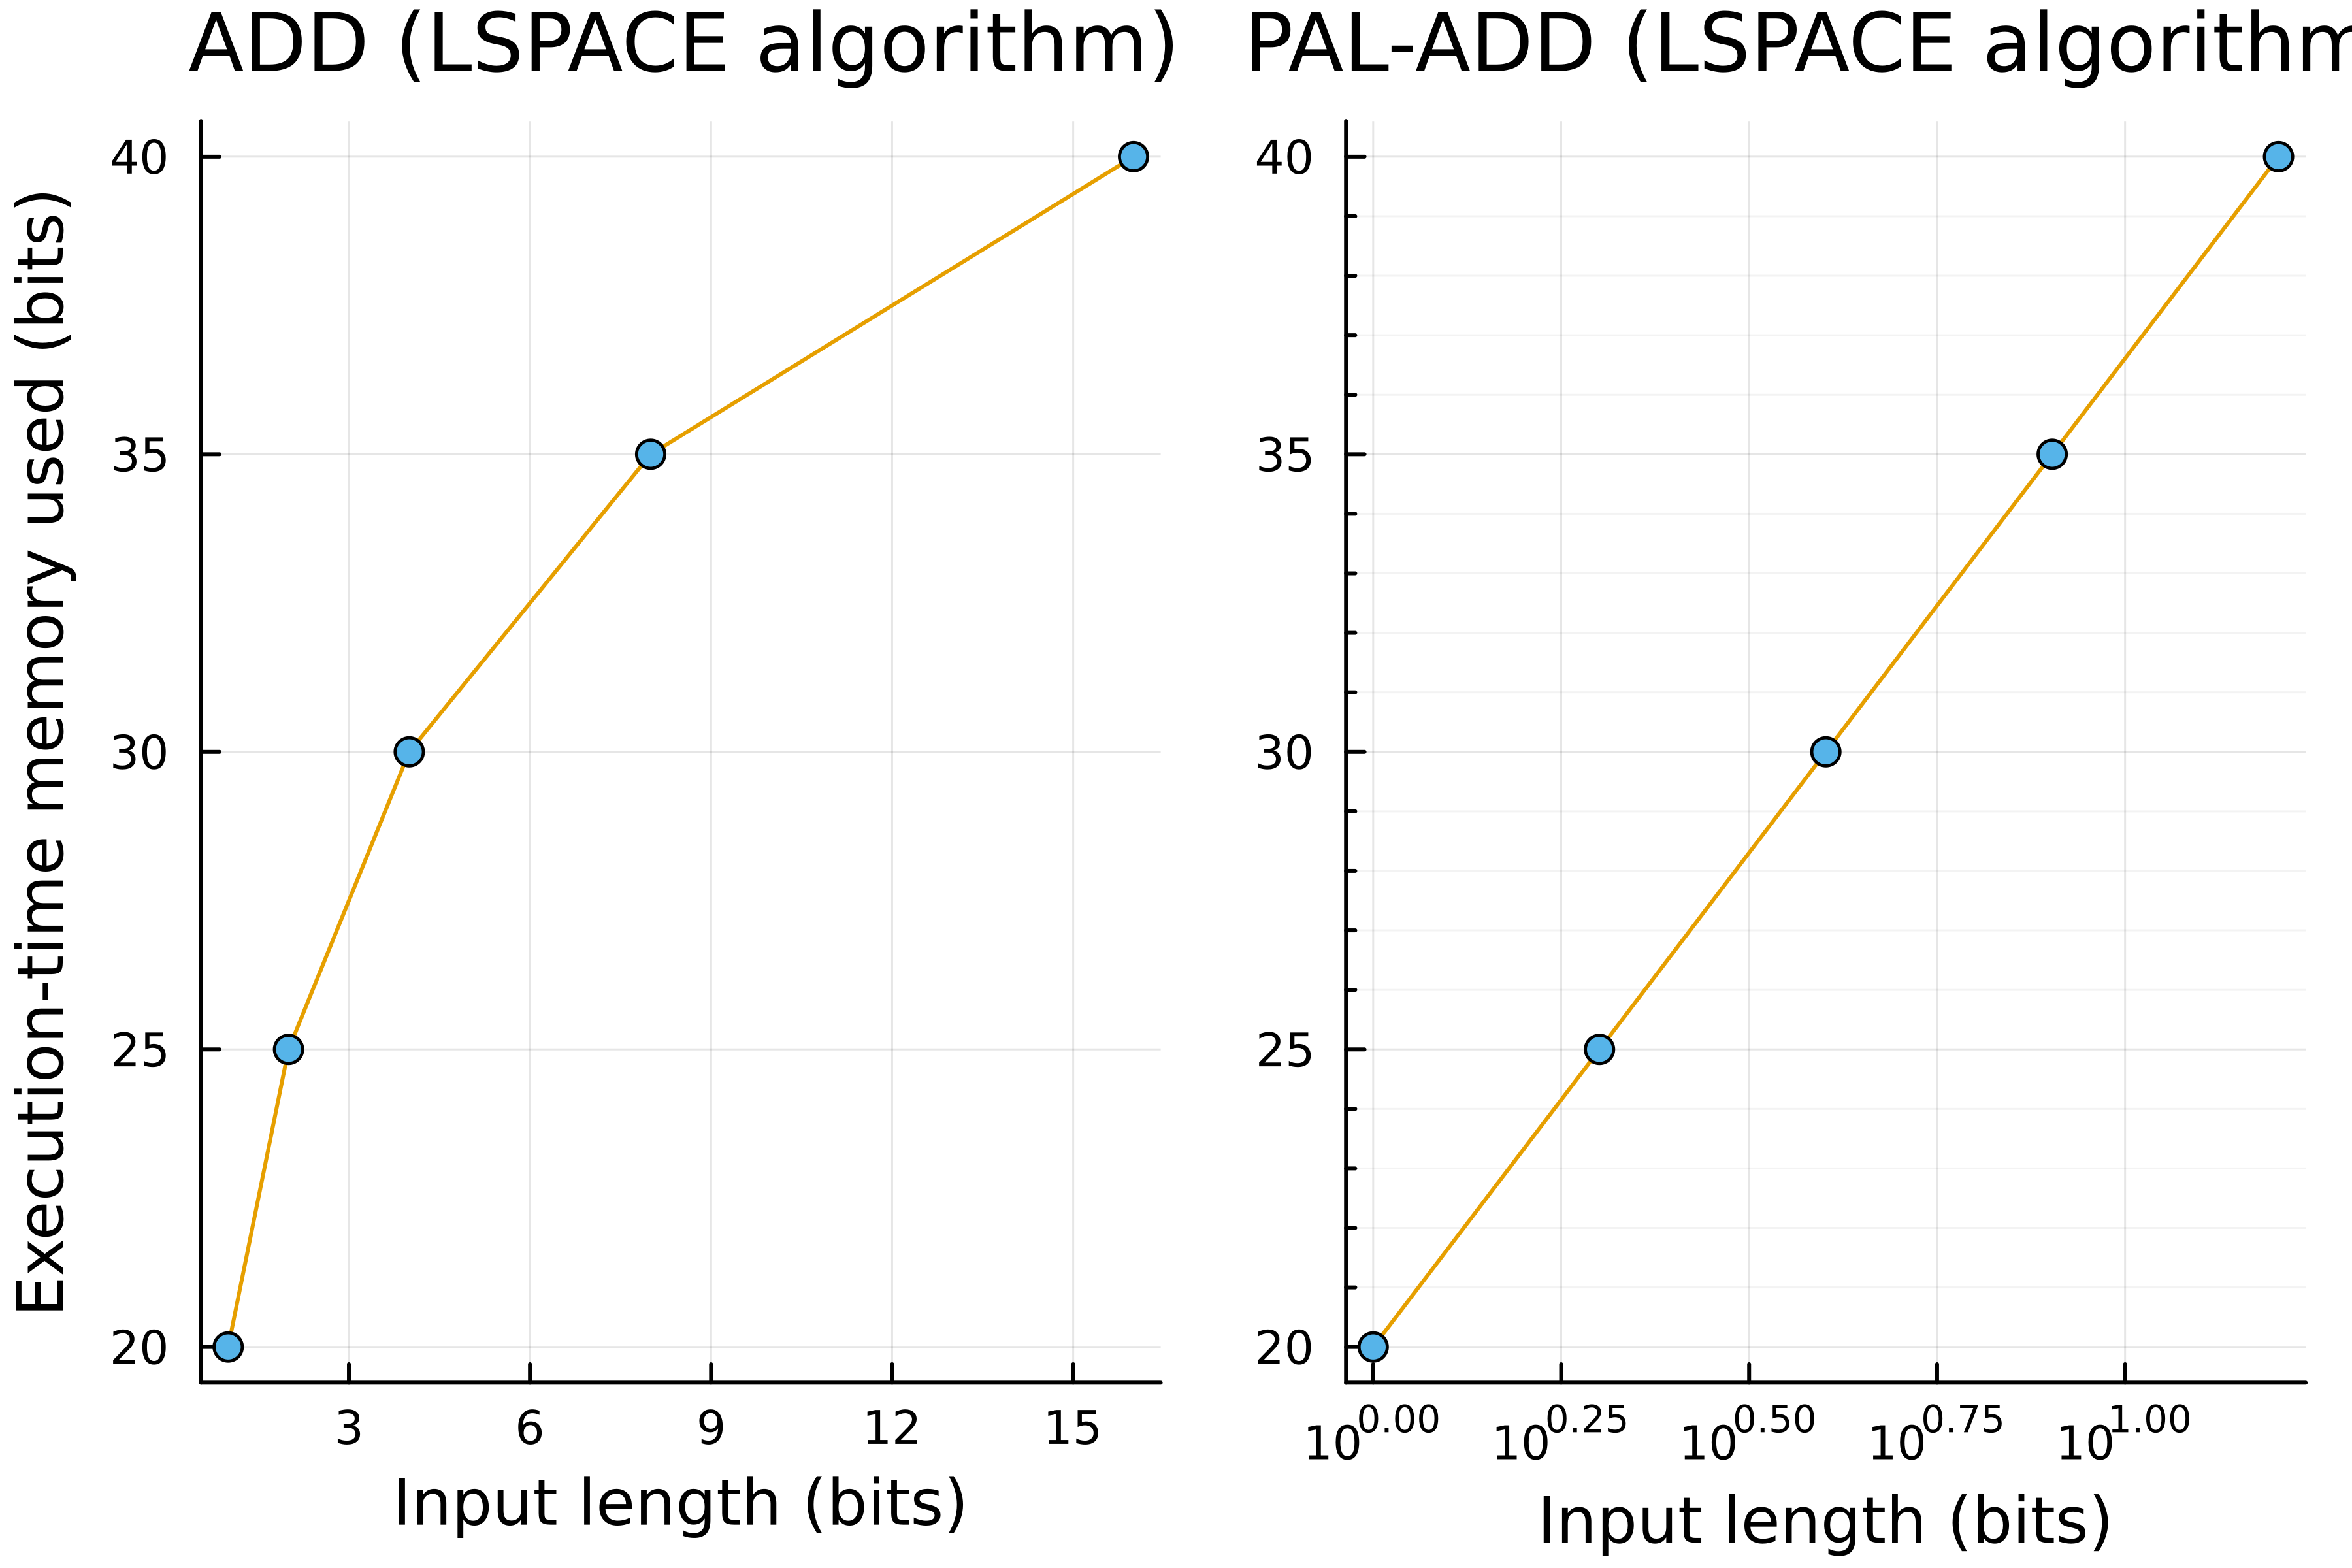
\includegraphics[width=\columnwidth]{PAL-ADD-(LSPACE-algorithm).png}
    \caption{Execution-time memory usage (bits) vs. input length (bits) for the LSPACE PAL-ADD algorithm given in Appendix \ref{app:palAdd}}
    \label{fig:palAdd}
\end{figure}

\newpage

\onecolumn

\appendix

\section{Munin example algorithms}
\subsection{Linear-space ADD algorithm}

\subsubsection{Pseudo-code}

\begin{lstlisting}
    function lin_add(x, y, z)
        a = x
        b = y
        c = z
        a += b
        if a != c
            return false
        end
        return true
    end
\end{lstlisting}

\subsubsection{Munin assembly code}

\lstinputlisting{../../examples/lin-add.asm}

\subsection{LSPACE ADD algorithm}

\subsubsection{Pseudo-code}

Note: it is assumed that the \lstinline|carry_flag| is set automatically when binary addition is performed and is set to \lstinline|false| at the start of each function.

\begin{lstlisting}
    function add(x, y, z)
        len = size_of(z)
        i = size_of(x)
        if i > len
            return false
        end
        i = size_of(y)
        if i > len_z
            return false
        end
        i = 0
        while i < len_z
            x_bit = get_nth_bit_of(x, i)
            y_bit = get_nth_bit_of(y, i)
            if carry_flag
                x_bit = add_bits(x_bit, 1)
            end
            x_bit = add_bits(x_bit, y_bit)
            z_bit = get_nth_bit_of(z, i)
            if x_bit != z_bit
                return false
            end
            i += 1
        end
        return true
    end
\end{lstlisting}

\subsubsection{Munin assembly code}

\lstinputlisting{../../examples/add.asm}

\subsection{LSPACE PAL-ADD algorithm}

\subsubsection{Pseudo-code}

Note: it is assumed that the \lstinline|carry_flag| is set automatically when binary addition is performed and is set to \lstinline|false| at the start of each function.

\begin{lstlisting}
    function pal_add(x, y)
        len = size_of(x)
        len_tmp = size_of(y)
        if len_tmp > len
            len = len_tmp
        end
        carry_on_last = carry_on_last_of_sum(x, y)
        i = 0
        while i < len
            i_bit = get_nth_bit_of_sum(x, y, i)
            j = len - i - 1 + carry_on_last
            j_bit = get_nth_bit_of_sum(x, y, j)
            if i_bit != j_bit
                return false
            end
            i += 1
        end
        return true
    end

    function get_nth_bit_of_sum(x, y, n)
        i = 0
        while i < n
            x_bit = get_nth_bit_of(x, i)
            y_bit = get_nth_bit_of(y, i)
            if carry_flag
                x_bit = add_bits(x_bit, 1)
            end
            x_bit = add_bits(x_bit, y_bit)
            i += 1
        end
        return x_bit
    end

    function carry_on_last_of_sum(x, y)
        len = size_of(x)
        len_tmp = size_of(y)
        if len_tmp > len
            len = len_tmp
        end
        i = 0
        while i < len
            x_bit = get_nth_bit_of(x, i)
            y_bit = get_nth_bit_of(y, i)
            if carry_flag
                x_bit = add_bits(x_bit, 1)
            end
            x_bit = add_bits(x_bit, y_bit)
            i += 1
        end
        if carry_flag
            return 1
        else
            return 0
        end
    end
\end{lstlisting}

\subsubsection{Munin assembly code}

\lstinputlisting{../../examples/pal-add.asm}

\newpage
\section{Munin assembly reference}

\begin{tabular}[H]{| p{0.12\linewidth} | p{0.12\linewidth} | p{0.12\linewidth} | p{0.12\linewidth} | p{0.35\linewidth} |}
   
    \hline
    \multicolumn{5}{| c |}{Munin assembly reference}\\
    \hline
    \hline
    Operator & Operand 1 & Operand 2 & Operand 3 & Description\\
    \hline
    \multicolumn{5}{| c |}{Assignment operaions}\\
    \hline
    \lstinline|set| & \lstinline|D| & \lstinline|S| & & Sets variable D equal to the value of S\\
    \lstinline|stl| & \lstinline|D| & \lstinline|S| & & Sets variable D equal to the length of S\\
    \lstinline|stnb| & \lstinline|D| & \lstinline|S| & \lstinline|N| & Sets variable D equal to the Nth bit of S\\
    \hline
    \multicolumn{5}{| c |}{Integer arithmetic operaions}\\
    \hline
    \lstinline|iadd| & \lstinline|D| & \lstinline|S| & & Sets variable D equal to the value of D + S\\
    \lstinline|isub| & \lstinline|D| & \lstinline|S| & & Sets variable D equal to the value of D - S\\
    \hline
    \multicolumn{5}{| c |}{Binary arithmetic operaions}\\
    \hline
    \lstinline|badd| & \lstinline|D| & \lstinline|S| & & Sets one-bit variable D equal to the value of the binary sum of one-bit D and one-bit S; sets carry flag\\
    \lstinline|bsub| & \lstinline|D| & \lstinline|S| & & Sets one-bit variable D equal to the value of the binary subtraction of one-bit D and one-bit S; sets the underflow flag\\
    \lstinline|bsr| & \lstinline|D| & \lstinline|S| & & Sets variable D equal to the value of D << S\\
    \lstinline|bsl| & \lstinline|D| & \lstinline|S| & & Sets variable D equal to the value of D >> S\\
    \hline
    \multicolumn{5}{| c |}{Comparison operaions}\\
    \hline
    \lstinline|cmp| & \lstinline|A| & \lstinline|B| & & Sets the equal flag if A == B ; sets the greater flag if A > B\\
    \lstinline|clf| & & & & Clears all flags\\
    \hline
    \multicolumn{5}{| c |}{Program flow operaions}\\
    \hline
    \lstinline|jmp| & \lstinline|D| & & & Jumps to line D\\
    \lstinline|end| & & & & Ends the program\\
    
    \hline

\end{tabular}

\end{document}
